\subsection*{Fase 6: Evaluación e interpretación}

En esta etapa se realizó la la evaluación e interpretación de los resultados obtenidos por el modelo \textit{k-means} visto en la fase anterior. Para ello, se utilizo el \textit{método del codo} y el \textit{método de la silueta} para determinar si el número de clusters generado por el modelo fue el adecuado. Podemos definir el coeficiente de la silueta como:

\begin{itemize}[label=]
	\item $a(x)=$ distancia promedio de $x$ a todos los demás puntos en el mismo cluster.\\
	\item $b(x)=$ distancia promedio de $x$ a todos los demás puntos en el cluster más cercano.
\end{itemize}

Dado esto, se dice que el coeficiente de la silueta para $x$ está dado por:

\begin{equation}
	s(x) = \frac{b(x)-a(x)}{max\left\lbrace a(x), b(x) \right\rbrace }
\end{equation}

\break
Donde el valor de $s(x)$ puede variar entre $-1$ y $1$. En donde, $-1$ es interpretado como un mal agrupamiento, $0$ como un resultado indiferente y $1$ como un buen agrupamiento \cite{Ramirez2018}. Por lo tanto, el coeficiente de la silueta para todo el agrupamiento es:

\begin{equation}
	SC = \frac{1}{N} \sum_{i = 1}^{N}s(x)
\end{equation}

En el caso del modelo \text{k-means} creado anteriormente, se obtuvo un valor de $k = 4$. Este valor fue comprobado por el método de la silueta obteniendo el resultado que se observa en la figura \ref{Silhouette}. En ella se puede observar que existen $4$ clusters cercanos a $1$ lo cual indica que el agrupamiento es aceptable. 

\begin{figure}[h!]
	\centering
	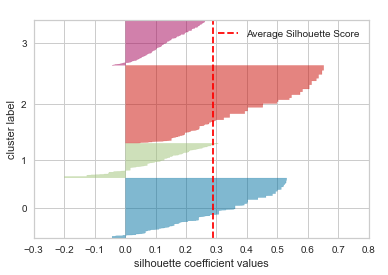
\includegraphics[width=1
	\linewidth]{IMAGENES/Silhouette}
	\caption{Método de la silueta para el modelo k-means.}
	\label{Silhouette}
\end{figure} 

Algo similar sucede con el \textit{método del codo}, el cual utiliza los valores de la inercia obtenidos tras aplicar el método \textit{k-means} a diferente número de clusters (desde $1$ a $N$ clusters), siendo la inercia la suma de las distancias al cuadrado de cada objeto del cluster a su centroide:

\begin{equation}
	inercia = \sum_{i = 0}^{N}  \parallel x_{i} - \mu  \parallel
\end{equation}

Una vez obtenidos los valores de la inercia tras aplicar el $k-means$ de $1$ a $N$ clusters, se representa en una gráfica lineal la inercia respecto del número de clusters. En esta gráfica se debería de apreciar un cambio brusco en la evolución de la inercia, teniendo la línea representada una forma similar a la de un brazo y su codo. El punto en el que se observa ese cambio nos indica el número óptimo de clusters a seleccionar para el conjunto de datos en cuestión \cite{Moya2022}. Dado lo anterior, en la figura \ref{Elbow} se observa que la inercia se produce en $k = 5 $ , lo cual indica que el modelo \textit{k-means} en cuestión tiene el numero de clusters adecuado. 

\begin{figure}[h!]
	\centering
	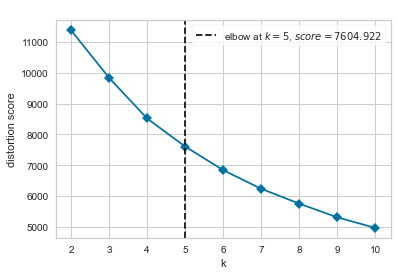
\includegraphics[width=1
	\linewidth]{IMAGENES/Elbow}
	\caption{Método del codo para el modelo k-means.}
	\label{Elbow}
\end{figure} 

Llegado a este punto, en la figura \ref{distribucion_total} se observa el la distribución obtenida para cada una de las variables en los 4 grupos generados en por el modelo \textit{k-means}, con base al conjunto de datos de morbilidad por cáncer de mama en el municipio de Pereira-Risaralda.

\begin{figure}[h!]
	\centering
	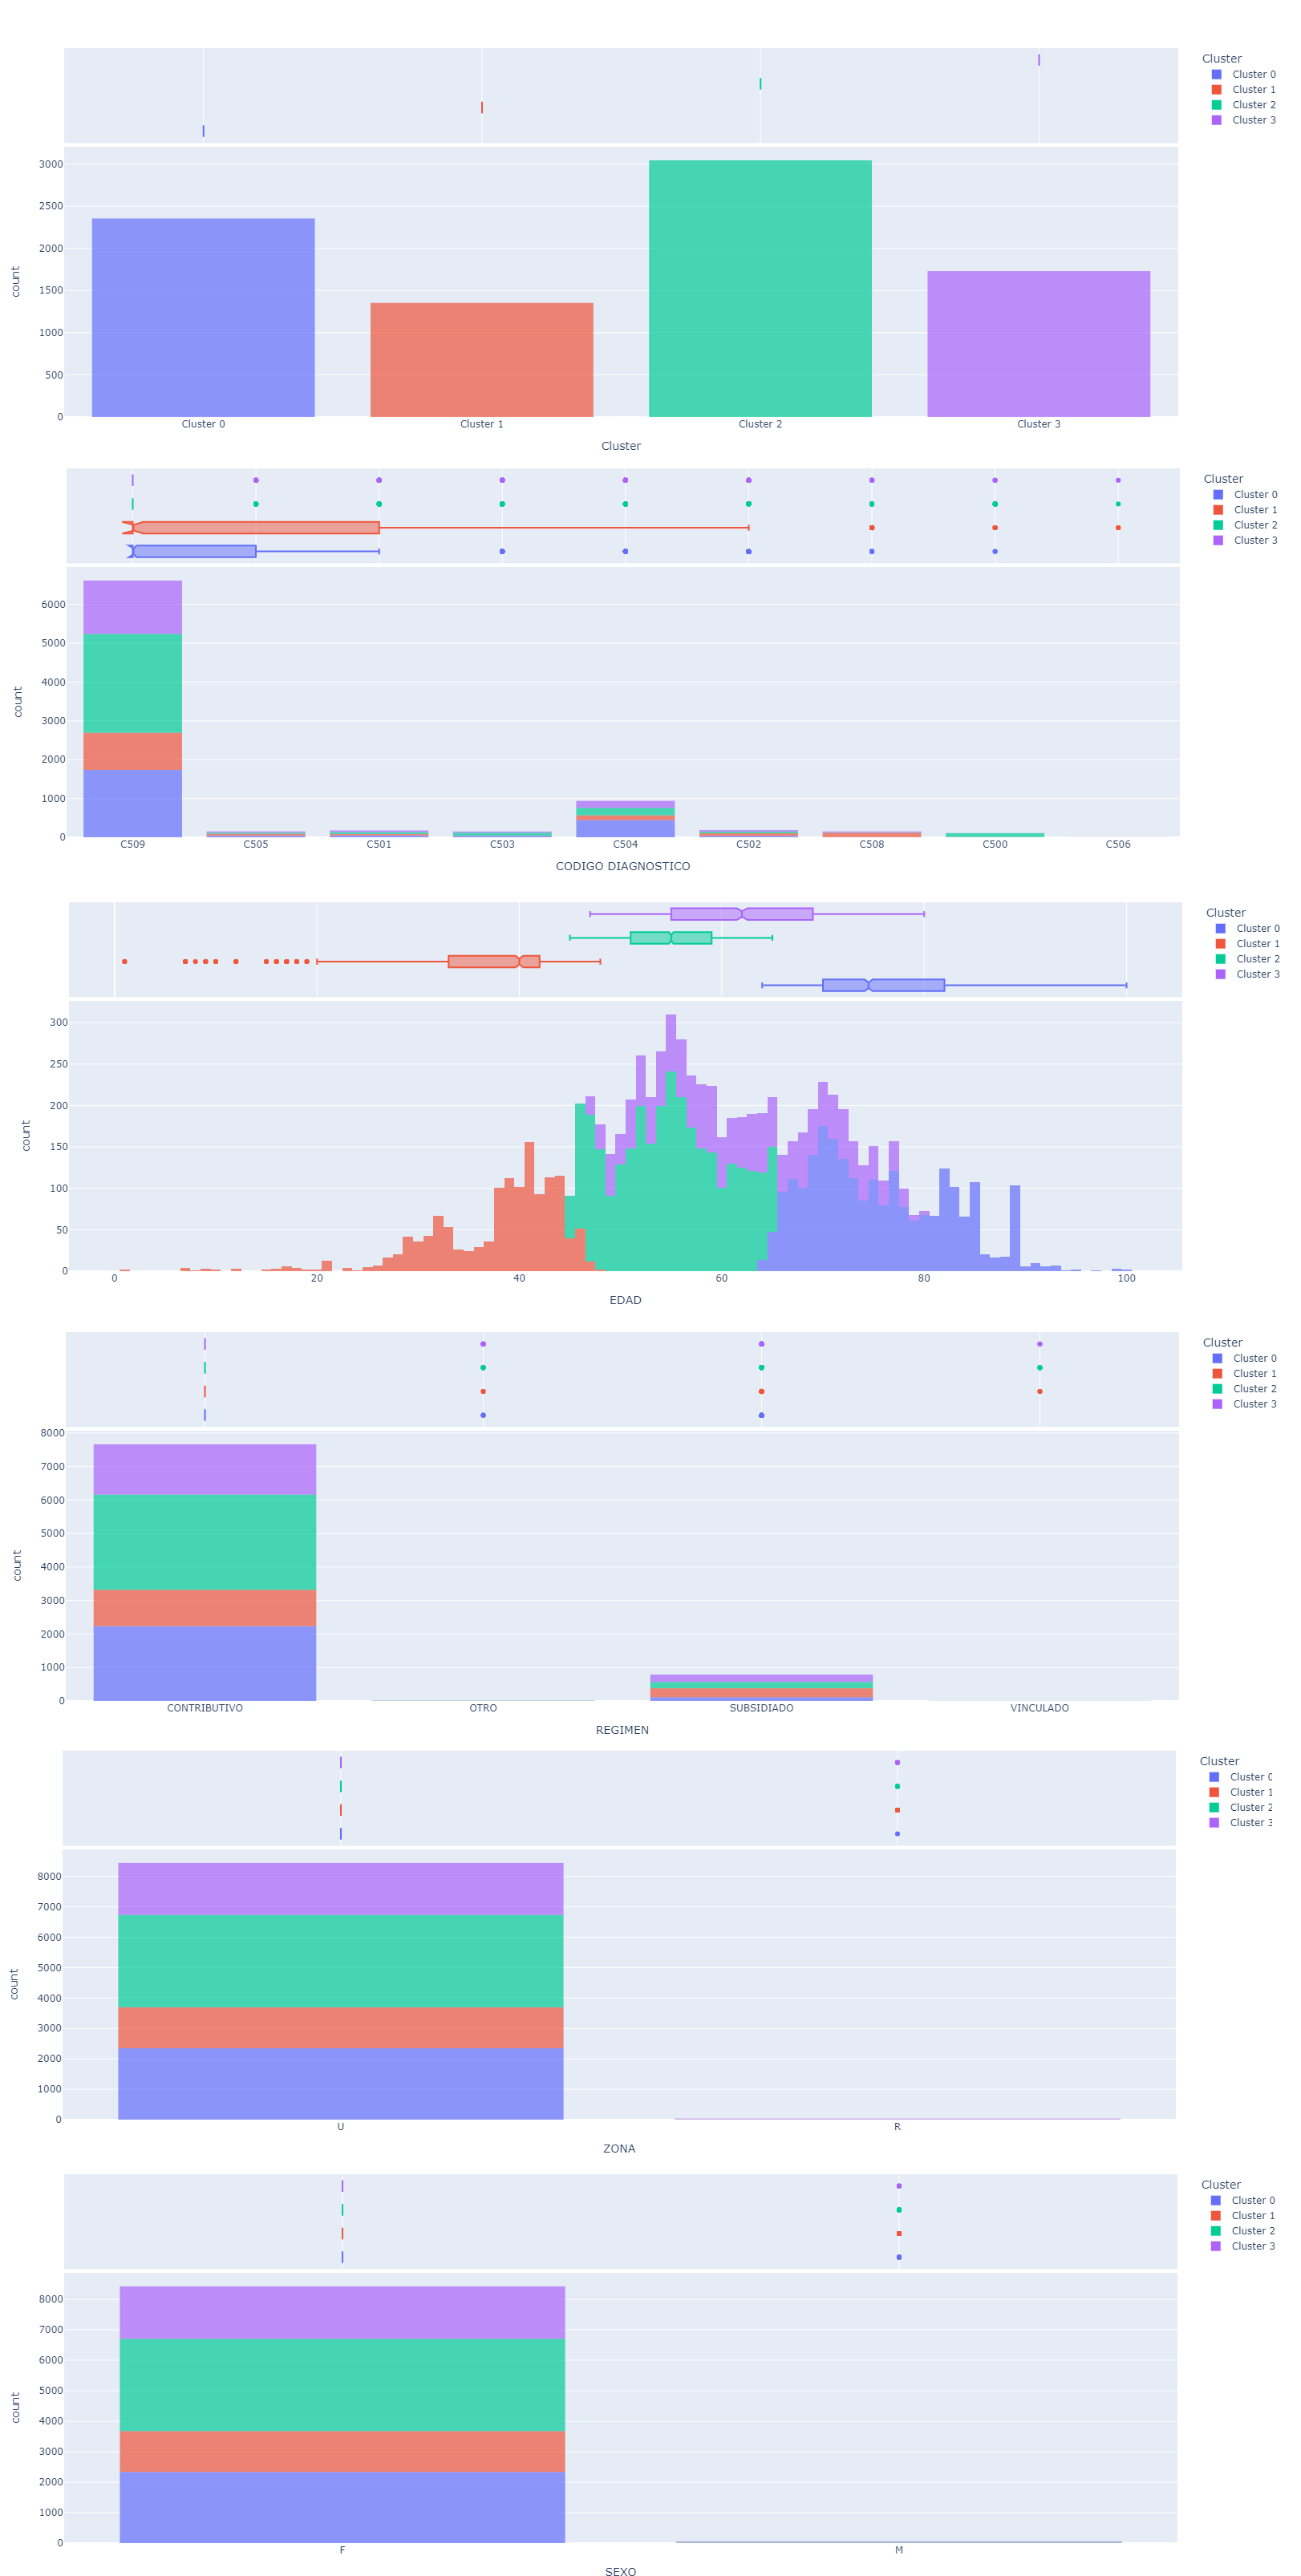
\includegraphics[width=1
	\linewidth]{IMAGENES/Distribucion_Total}
	\caption{Distribución en 4 clusters de 8481 registros.}
	\label{distribucion_total}
\end{figure} 

Interpretando los resultados obtenidos, es posible afirmar que el cáncer con código topográfico de $C509$ relacionado con múltiples tumores en diferentes sub-sitios dentro de la mama, esta presente en todos los grupos generados por el modelo \textit{k-means}. De igual forma, los sujetos de genero femenino que están afiliados a un régimen de salud contributivo y que habitan en zonas urbanas también están presentes en cada uno de los clusters. Sin embargo, aunque esta información se determino en el \textit{análisis exploratorio de datos} de la fase 1, se encontró un patrón interesante en la variable edad. Como se puede observar en la figura \ref{distribucion_total}, la morbilidad por cáncer de mama puede ser determinada como: Severa para edades entre 51 y 59 años, alta para edades entre 70 y 82 años, media para edades entre 55 y 69 años y baja para edades entre 33 y 42 años. De estos resultados es posible inferir que el cáncer de mama no presenta un comportamiento directamente dependiente con la variable edad, es decir no necesariamente la morbilidad por esta enfermedad se desarrolla en la medida en que las mujeres envejecen, por el contrario presenta su punto de letalidad mas alto en las mujeres risaraldenses con 55 años de edad. Adicionalmente, aunque el tipo de cáncer con código topográfico de $C504$ relacionado al Cuadrante superior externo (UOQ) de la mama, no estuvo contenido en ninguno de los cluster generados por el modelo se puede determinar que presento un numero de muertes significativas para mujeres con rango de edad 70 y los 82 años edad.
